\chapter{Collecte et étude statistique}
\epigraph{Economists and agronomists are locked in debate about likely
future yields. Since the method of the economists is to predict
future outcomes from past performance, economists expect
success to continue. And since for the scientists future success
depends on discoveries they will have to make and do not now
know how to make, the scientists are doubtful. At its core, this is
a disagreement about the pace of technical change.}{Robert
Socolow}	
\cleardoublepage
\newcommand{\reels}{\mathbb{R}}
	\section{Collecte des données}
	\subsection{Compréhension des données locales\protect\footnote{Données disponibles au sein du portail Business Intelligence de l'OCP}}
	Au sein du portail Business intelligente de l'OCP on constate deux différentes formes de données, la première est structurée dans des Data-Mart dont une sortie de requête est présentée dans la figure \ref{fig:DMOCP}.
	 	\begin{figure}[h]
	    		\centering
    			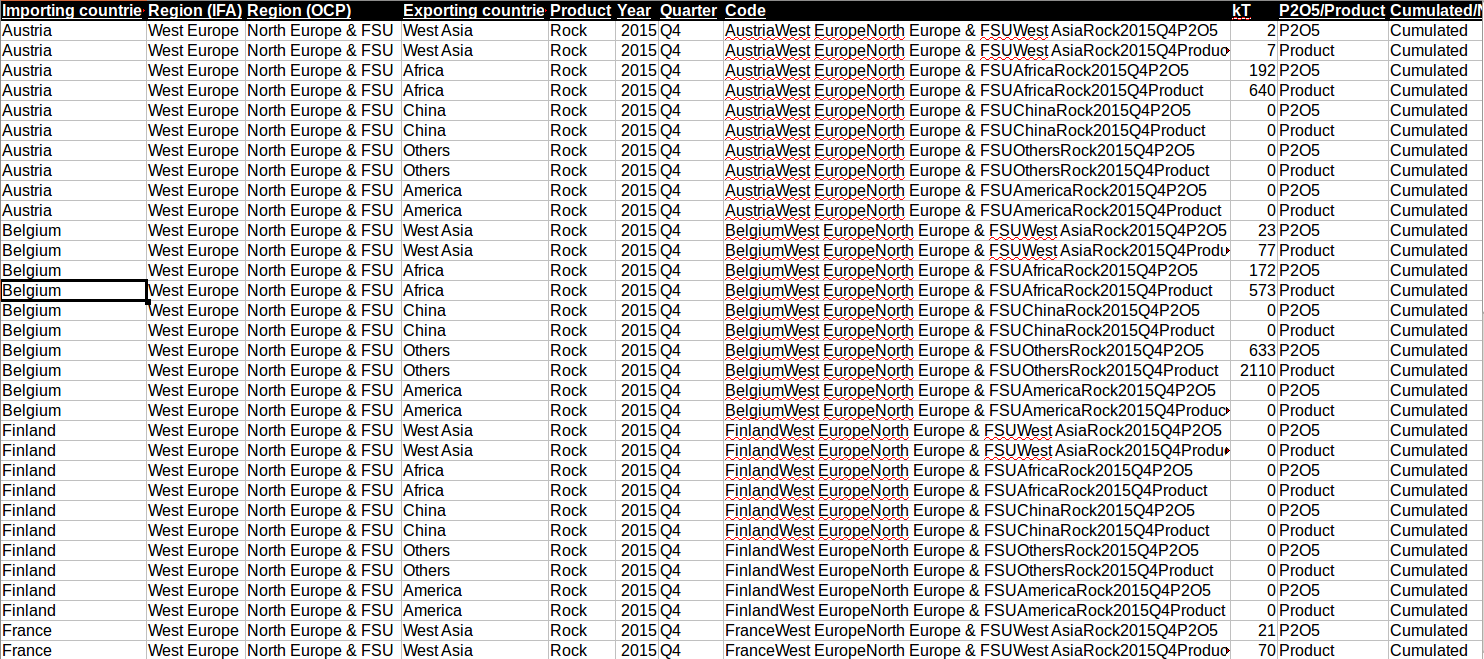
\includegraphics[scale=0.35]{Table}
	    		\caption{Example d'une sortie de requête sur le Data-Mart}
	    		\label{fig:DMOCP}
	\end{figure}
	\par
	Ceci est notre format de données cible et présente:
	\begin{itemize}
	\item L'avantage d’offrir le maximum de flexibilité pour le requêtage, et d'être de grande qualité en terme de disponibilité et de veracité, puisque celui-ci a été soigneusement introduit à la main\footnote{À travers une lecture "humaine" des .pdf présentés plus bas}.
	\item L’inconvénient d'être prohibitif en temps et en ressources humaines. En effet, nous avons constaté un retard data de fin décembre 2013 par rapport aux derniers .pdf reçus par l'OCP.
	\end{itemize}
	La seconde a une forme non structurée vis-à-vis de notre besoin -des fichiers .pdf (figure \ref{fig:IFA-PDF})- et qui présente:
	\begin{itemize}
	\item L'avantage d’être a jour, exhaustive et certifie par un organisme international (IFA\footnote{International Fertilizer Association: Association Internationale des Fertilisants})
	\item L’inconvénient d’être flexible pour la lecture humaine mais ne présentant pas une grammaire machine formelle rendant possible une analyse syntaxique, comme en  la figure \begin{huge}
	A faire
	\end{huge}
	\end{itemize}
	\par
	\begin{figure}[H]
	    		\centering
    			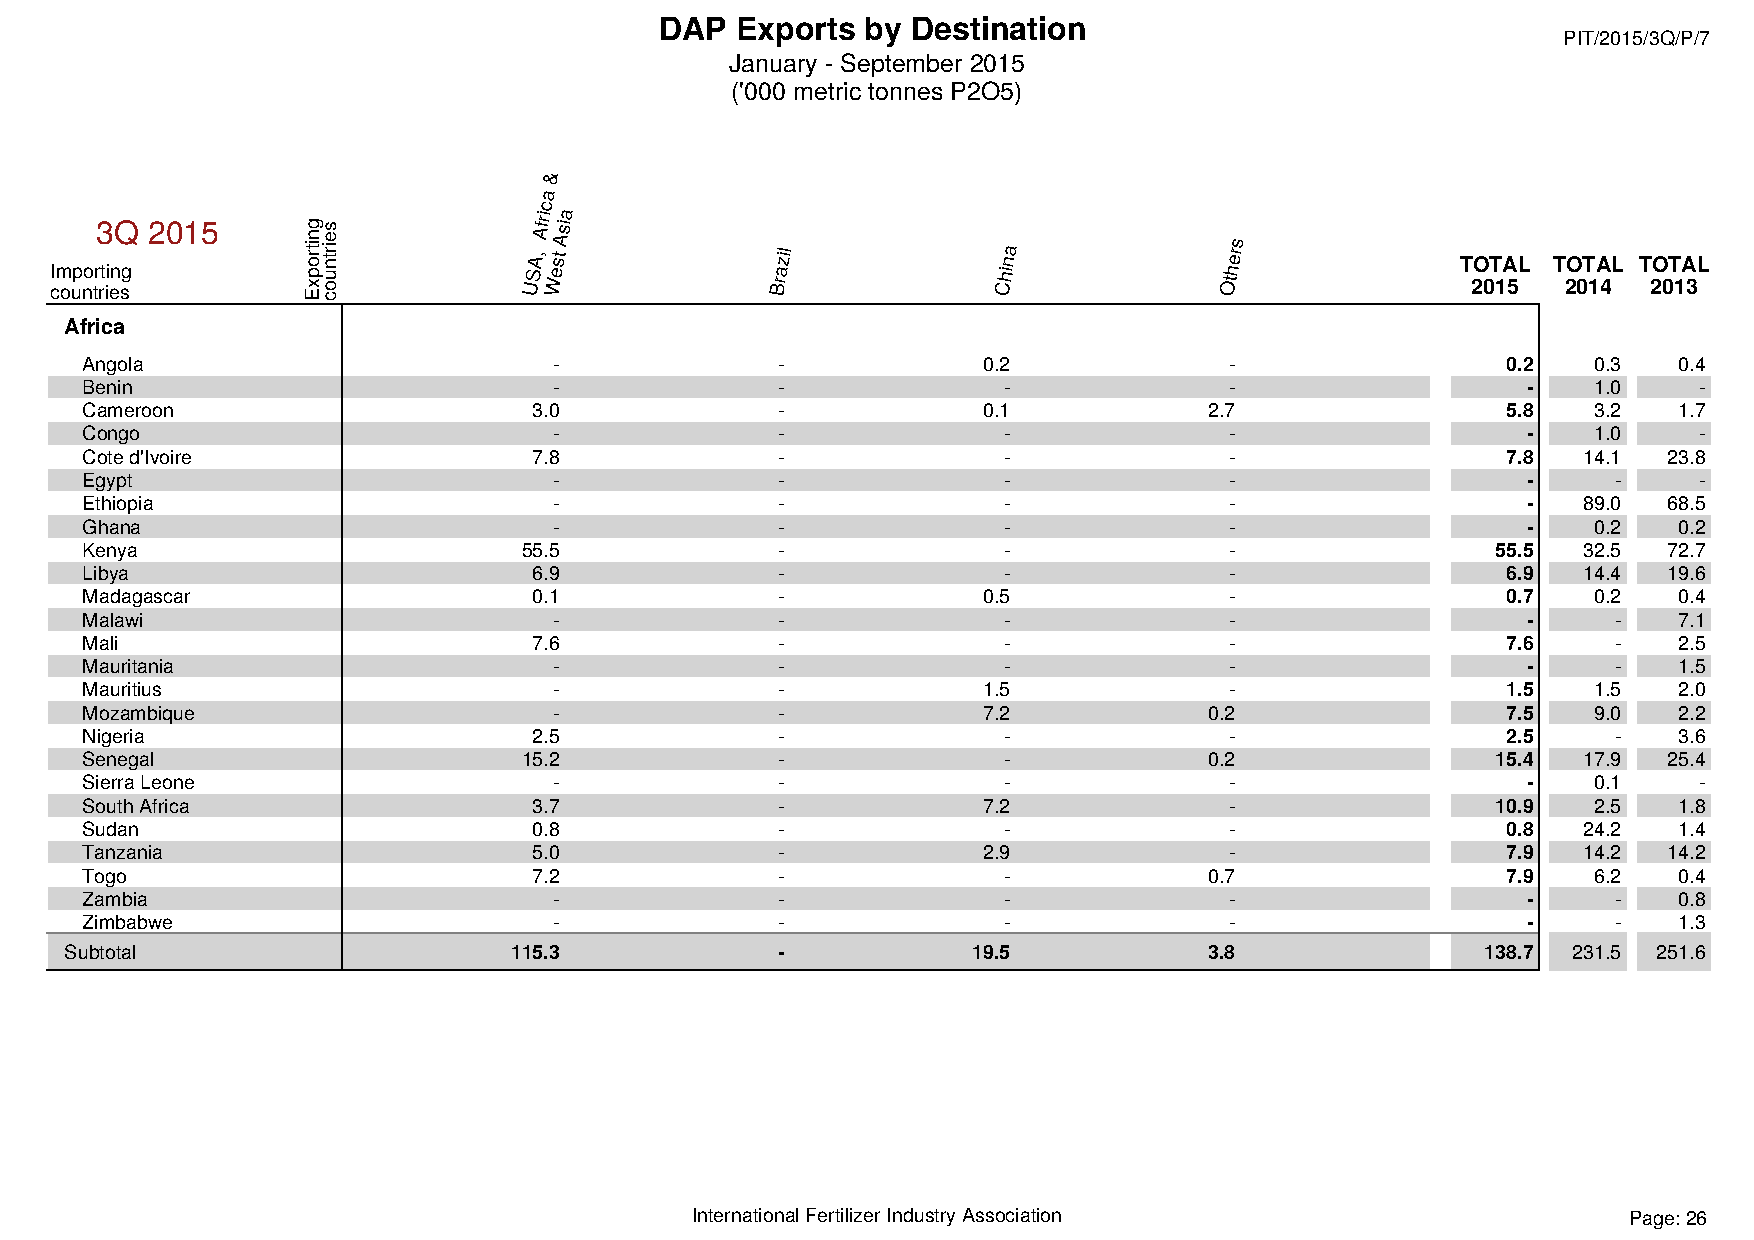
\includegraphics[scale=0.6]{IFA_EX}
	    		\caption{Example d'une trade Matrix dans le rapport Trimestriel de l'IFA}
	    		\label{fig:IFA-PDF}
	\end{figure}
	\par
	Dans notre cas mous sommes intéressés par les données d'import et export des produits phosphatés, cette donnée existante dans le portail est non structuré, elle est sous format PDF.
	\subsubsection{Analyse des PDFs contenant les trades Matrix}
		
	\paragraph{Contraintes:}
	\begin{itemize}
		\item Il faut distinguer et localiser les Trades Matrix des autres formes de données contenues dans ce document.
		\item L'extraction manuelle des structures de table d'un fichier PDF consomme énormément de temps et d'energie.
		\item Après l'extraction, Il faut transformer ces trades Matrix En des trades table pour faciliter le requettage.
	\end{itemize}
	\subsubsection{Conception de la solution}
	\subsection{Extension des données aux banques externes}
	Comme rappelé dans la section \ref{CGP}. Les travaux de nos prédécesseurs dans leurs efforts de moderniser le système d'information se sont arrêtés à automatiser l'archivage des données se rapportant aux historiques de ventes en terme de prix et volumes en un premier lieu\cite{CHEMLAL} avant de concevoir le socle OLAP\footnote{le traitement analytique en ligne (OnLine Analytical Processing, OLAP) est un type d'application informatique orienté vers l'analyse sur-le-champ d'informations selon plusieurs axes, dans le but d'obtenir des rapports de synthèse} dans la vue de générer des rapports synthétiques concernant les historiques des échanges du marché des phosphates ensuite\cite{NACER}.
	\par
	L'étendue des données disponibles au sein du système d'information de l'OCP ne pouvant donner qu'une vue réduite de la situation du marché et ne peuvent de par leur définition révéler les structures socio-économiques,  et de politiques agraires sous-jacentes aux demandes en produits phosphatés, nous nous attellerons à la tâche d'enrichir cette base de données historiques par des données quantitatives concernant les pays du monde.
	\par
	Nous décrivons dans ce qui suit ce processus. 
	\subsubsection{Énumération, recherche et extraction des données depuis des banques WEB}
		Guidés par nos lectures bibliographiques résumées dans les sections \ref{read1} et \ref{read2}, nous nous fixons l'objectif de récolter les indicateurs de politiques agraires et socioéconomiques suivants:
	\paragraph{Énumération et définitions des variables souhaitées }
	\begin{itemize}
		\item \textbf{ Access to electricity, rural (\% of rural population):} Fraction de paysans ayant accès à l'électricité.
		\item \textbf{ Access to non-solid fuel, rural (\% of rural population):} Fraction de paysans ayant accès aux fuels non solides.
		\item \textbf{ Account at a financial institution (\% age 15+):} Fraction de personnes âgées de +15 ans ayant un compte chez une institution bancaire.
		\item \textbf{ Net enrollment rate, primary (\% of primary school age children):} Fraction d'enfants scolarisés.
		\item \textbf{ Net national income per capita (constant 2005 US\$):} PIB\footnote{Produit intérieur brut, un des agrégats majeurs des comptes nationaux, il vise à quantifier — pour un pays et une année donnés — la valeur totale de la « production de richesse » effectuée par les agents économiques résidant à l’intérieur de ce territoire (ménages, entreprises, administrations publiques).} par habitant, inflation ajustée au dollar US fin 2005.
		\item \textbf{ Literacy rate, adult total (\% of people ages 15 and above):} Fraction de personnes alphabétisées âgées de +15ans.
		\item \textbf{ Agricultural irrigated land (\% of total agricultural land):} Fraction de terres irriguées parmi les terres exploitées pour l'agriculture.
		\item \textbf{ Agricultural land (\% of land area):} Fraction des terres agricoles de la surface totale du pays.
		\item \textbf{ Agricultural tractors per 100 sq. km of arable land:} Nombre de tracteurs par 100 km² de terres arables.
		\item \textbf{ Agriculture, value added (\% of GDP):} Fraction de la valeur ajoutée agricole du PIB.
		\item \textbf{ Agriculture value added per worker (constant 2005 US\$):} Valeur ajoutée agricole par ouvrier agricol, inflation ajustée au dollar US fin 2005.
		\item \textbf{ All education staff compensation, total (\% of total expenditure in public institutions):} Fraction des dépenses en éducation des dépenses en institutions publiques.
		\item \textbf{ Annual freshwater withdrawals, agriculture (\% of total freshwater withdrawal):} Fraction du volume d'eau utilsée à des fins agricoles de la totalité de l'eau consommée.
		\item \textbf{ Arable land (\% of land area):} Fraction de terres arables de la surface totale du pays.
		\item \textbf{ Arable land (hectares per person):} Nombre d'hectares de terres arables par personne.
		\item \textbf{ Birth rate, crude (per 1,000 people):} Nombre de naissances par 1000 personnes.
		\item \textbf{ Cereal yield (kg per hectare):} Rendement des céréales en kilogramme par hectare.
		\item \textbf{ Commercial bank branches (per 100,000 adults):} Nombre d'agences bancaires par 100,000 adultes.
		\item \textbf{ Consumer price index (2010 = 100):} L'indice des prix à la consommation (IPC) mesure l'évolution du niveau moyen des prix des biens et services consommés par les ménages, pondérés par leur part dans la consommation moyenne des ménages. Harmonisé pour permettre une comparaison entre les pays à fin 2010.
		\item \textbf{ Cost to export (US\$ per container):} Coût en Dollars US de l'export d'un conteneur de marchandises.
		\item \textbf{ Cost to import (US\$ per container):} Coût en Dollars US de l'import d'un conteneur de marchandises.
		\item \textbf{ Crop production index (2004-2006 = 100):} 
		L'indice de production des cultures montre la production agricole pour chaque année par rapport à la période de base de 2004 à 2006. Cet indice porte sur l'ensemble des cultures à l'exception des cultures fourragères. Les regroupements par région et par revenu des indices de production de la FAO sont calculés à partir des valeurs sous-jacentes en dollars US et normalisés par rapport à la période de référence de 2004 à 2006.
		\item \textbf{ Droughts, floods, extreme temperatures (\% of population, average 1990-2009):} Pourcentage moyen annuel entre 1990 et 2009 de la population affectée par les catastrophes naturelles classifiées comme sécheresses, inondations et évènements climatiques extrêmes.
		\item \textbf{ Employment in agriculture (\% of total employment):} Fraction des ouvriers agricoles de l'ensemble des employés.
		\item \textbf{ Food production index (2004-2006 = 100):} L'indice de production alimentaire porte sur les cultures vivrières qui sont considérées comme comestibles et qui contiennent des nutriments et normalisées par rapport à la période de référence de 2004 à 2006.
		\item \textbf{ GDP per capita (constant 2005 US\$):} PIB par habitant. Inflation ajustée à fin 2005.
		\item \textbf{ Household final consumption expenditure (constant 2005 US\$):}  La consommation privée désigne la valeur marchande de tous les biens et services, y compris les produits durables achetés par les ménages.
		\item \textbf{ Lending interest rate (\%):} Le taux d'intérêt perçu par les banques sur les prêts accordés aux clients.	
		\item \textbf{ Life expectancy at birth, total (years):} L'espérance de vie à la naissance indique le nombre d'années qu'un nouveau-né devrait vivre si les règles générales de mortalité au moment de sa naissance devaient rester les mêmes tout au long de sa vie.
		\item \textbf{ Livestock production index (2004-2006 = 100):} L'indice de production animale comprend la production de viande et de lait de toutes sources, les produits laitiers tels que le fromage, les œufs, le miel, la soie brute, la laine ainsi que les peaux et les cuirs.
		\item \textbf{ Logistics performance index:} La note globale de l'indice de performance de la logistique reflète les perceptions relatives à la logistique d'un pays basées sur l'efficacité des processus de dédouanement, la qualité des infrastructures commerciales et des infrastructures de transports connexes, la facilité de l'organisation des expéditions à des prix concurrentiels, la qualité des services d'infrastructure, la capacité de suivi et de traçabilité des consignations et la fréquence avec laquelle les expéditions arrivent au destinataire dans les délais prévus. L'indice varie continuellement de 1 à 5 et la note la plus élevée représente la meilleure performance.
		\item \textbf{ Low-birthweight babies (\% of births):} Fraction des nouveau-nés pesant moins de 2 500 grammes des naissances totales.
		\item \textbf{ Net migration:} Nombre d'immigrants total moins le nombre d'émigrants annuel, comprenant à la fois les citoyens et les non citoyens.
		\item \textbf{ Permanent cropland (\% of land area):} Fraction des terres occupées par des cultures pour de longues périodes et qui doivent être replantées après chaque récolte de la surface totale du pays.
		\item \textbf{ Population density (people per sq. km of land area):} Densité des habitants en personne par km².
		\item \textbf{ Population growth (annual \%):} Croissance relative annuelle de la population.
		\item \textbf{ Rural population (\% of total population):} Fraction rurale de la population.
		\item \textbf{ Rural poverty gap at national poverty lines (\%):} L'écart de pauvreté par rapport au seuil national de la pauvreté en milieu rural est le manque à gagner pour remonter au-dessus du seuil de la pauvreté (en considérant que les non pauvres ont un manque à gagner de zéro) exprimé en pourcentage du seuil national de la pauvreté en milieu urbain.Cette mesure témoigne à la fois de l'ampleur de la pauvreté et de sa fréquence.
		\item \textbf{ Unemployment, total (\% of total labor force):} Fraction de la population active qui est sans emploi mais qui est disponible pour et à la recherche d'un emploi.
		\end{itemize}
	\paragraph{Recherche des sources WEB des variables souhaitées \newline}
	\par
	\begin{Huge}{ Liste des cibles (sites web et bases de données publiques) du Crawling }
		\end{Huge}
	\paragraph{Extraction et formatage des variables souhaitées \newline}\label{crawl}
	\par
	 \begin{Huge}{ Workflow du  Crawling }
	 		\end{Huge}
	\subsubsection{Élagage des données externes}
	Cette section s’intéresse à l'application des forêts de décisions aléatoires à des fins de sélection de variables. Le but ici est double : d'abord introduire le comportement de l'indexation de l'importance des variables en utilisant les forêts aléatoires et l'utiliser pour proposer un algorithme à deux phases pour la sélection de variables à la base de leur importance.\par
	La stratégie générale se résume en un classement des variables exogènes\footnote{à savoir les variables externes "crawlées" dans la section \ref{crawl}.} en utilisant le score d'importance de ces variables introduit par les forêts aléatoires puis une sélection ascendante itérative des variables.
	\paragraph{Introduction aux forêts de décision aléatoires\newline}
	Les FA\footnote{Forêts aléatoires} est un algorithme populaire et très efficient basé appartenant aux méthodes d'agrégation pour les problèmes de régression et de classification, introduit par Breiman\cite{BREI01}, et apparaît dans les application de 'Machine Learning'\footnote{L'apprentissage automatique ou apprentissage statistique (machine learning en anglais), champ d'étude de l'intelligence artificielle, concerne la conception, l'analyse, le développement et l'implémentation de méthodes permettant à une machine (au sens large) d'évoluer par un processus systématique, et ainsi de remplir des tâches difficiles ou impossibles à remplir par des moyens algorithmiques plus classiques.} à la fin du dernier millénaire\cite{DITRI99}. Les FA deviennent de plus en plus populaires et semblent être très robustes dans beaucoup d'applications bien qu'ils ne soient pas clairement théorisés mathématiquement\cite{BIA08}.
	\par
	Considérons un ensemble d'apprentissage ${L_n = \{(X_1, Y_1),...,X_n, Y_n)\}}$ de \textit{n} observations i.i.d.\footnote{indépendantes identiquement distribuées} d'un vecteur aléatoire (X,Y). Le vecteur ${X_i = (X_i^1,...,X_i^p)}$ contient les variables exogènes, $X_i \in \reels^p $ et $Y_i \in \reels $, une réponse numérique. Pour les problèmes de regression, nous supposons que $ \exists$ S $\forall$ i $ Y_i=S(X_i)+\varepsilon$ où E[$\varepsilon$|X] = 0 et \textbf{S} est appellée fonction de regression. Les FA est une stratégie de construction d'un modèle \textit{ê(x)} estimant la fonction de regression.
	\par
	Les méthodes d’agrégation consistent à agréger un nombre \textit{B} d’estimateurs $ê_1,...,ê_\textit{B}$ : ${ê(x) = ê_B(x) =  \frac{1}{B} \sum_{i=1}^{B} ê_i}$. On considère l’erreur quadratique moyenne d’un estimateur \textit{ê} et sa décomposition biais-variance :
	\begin{center}
	${E[(ê(x)-S(x))^2] = (E[ê(x)] - S(x))^2 + Var(ê(x))}$
	\end{center}
	Si on suppose les régrésseurs $ê_1,...,ê_B$ i.i.d on a :
	\begin{center}
		$E[ê(x)] = E[ê_1(x)]$ et $Var(ê(x)) = \frac{1}{B} Var(ê_1(x)$
	\end{center}
	Le biais de l’estimateur agrégé est donc le même que celui des $ê_k(x)$ mais la variance diminue. Bien
	entendu, en pratique il est quasiment impossible de considérer des estimateurs $ê_k(x)$ indépendants
	dans la mesure où ils dépendent tous du même échantillon \textit{$L_n$} . L’approche des FA consiste à
	tenter d’atténuer la dépendance entre les estimateurs que l’on agrège en les construisant sur des
	échantillons bootstrap\footnote{Ré-échantillonnage}. Nous référerons le lecteur à l'annexe A, pour une démonstration.
	\par
	Le principe des FA est de combiner plusieurs arbres ($ê_i$) de décision CART\cite{BREI84} en utilisant plusieurs échantillons bootstrap de l'ensemble d'apprentissage \textbf{$L_n$} et de choisir aléatoirement à chaque nœud un sous-ensemble de \textit{k} variables exogènes $X_i$.
	
	\par
	 En comparaison avec le modèle CART qui lui procède à une phase de construction de l'arbre suivie d'une phase d'élagage, deux différences sont à relever. D'abord, à chaque nœud, un nombre paramètre (dénoté \textit{k}\footnote{L'autre paramètre des FA étant \textit{B}, le nombre d'arbres dont la forêt.}) de variables exogènes sont choisies aléatoirement et la meilleure variable pour la subdivision du nœud est choisie parmi celles-ci seulement. Ensuite, aucun élagage n'est introduit: tous les arbres de la forêt sont maximaux.\par
	Le principe de CART est de partitionner récursivement l’espace engendré par les variables explicatives (ici $\reels^p$) de façon dyadique. Plus précisément, à
	chaque étape du partitionnement, on découpe une partie de l’espace en deux sous parties selon une variable $X_j$ comme le montre la figure \ref{fig:CART}.
	\begin{figure}[h]
	    		\centering
	    		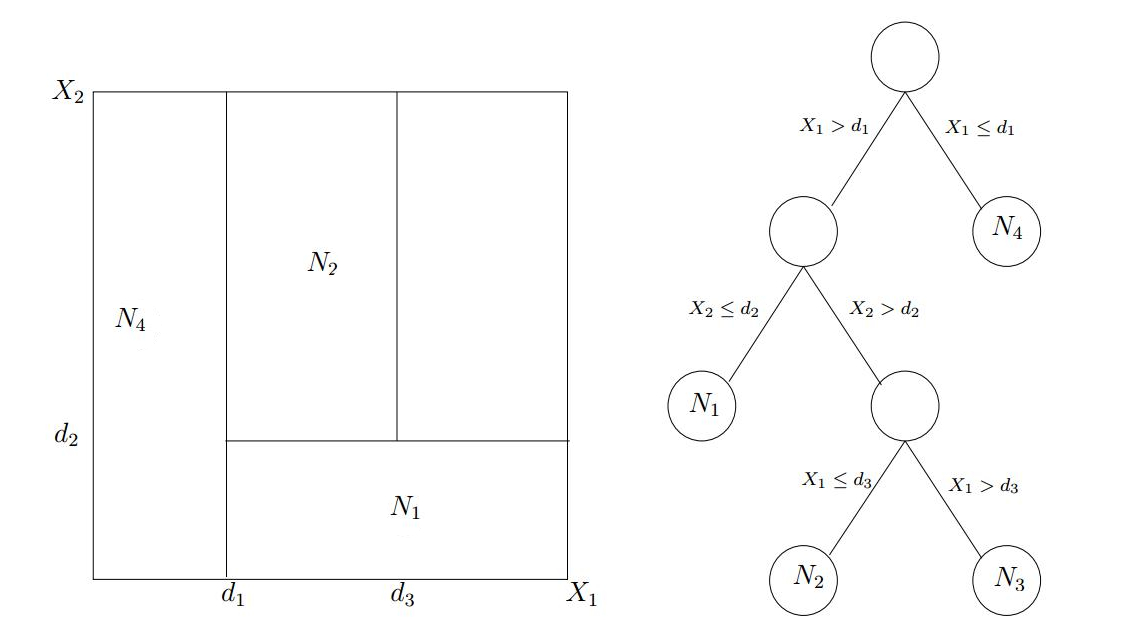
\includegraphics[scale=0.35]{Cart}
	    		\caption{Arbre CART}
	    		\label{fig:CART}
	\end{figure}
	\par
	Les coupures sont choisies de manière à minimiser une fonction de coût particulière. A chaque étape, on cherche la variable $X_j$ et le réel \textit{d} qui minimisent la variance des nœuds fils dans les problèmes de régression. Les arbres sont ainsi construits jusqu’à atteindre une règle d’arrêt. Par exemple, on ne découpe pas un nœud qui contient moins de 5 observations comme y procède le package \textbf{\textit{randomForest}} du langage \textbf{R}.
	\par
	Nous avons vu dans la section précédente que l'agrégation à laquelle procèdent les FA est d’autant plus performante que la corrélation entre les prédicteurs agrégés  (arbres CART) est faible. Afin de diminuer cette corrélation, Breiman\cite{BREI01} propose de rajouter une couche d’aléa dans la construction des
	prédicteurs. Plus précisément, à chaque étape de CART, \textit{k} variables sont sélectionnées aléatoirement parmi les \textit{p} et la meilleure coupure est sélectionnée uniquement sur ces \textit{k} variables : \par
	\textbf{Algorithme Forêts aléatoires}
	\begin{itemize}
	\item[\textbf{Entrées:}]
	\item x, une nouvelle observation à prévoir.
	\item \textit{$L_n$}, l'échantillon.
	\item \textit{B}, le nombre d'arbres.
	\item \textit{k} $\in \mathbb{N}^* $, le nombre de variables candidates pour découper un nœud.
	\end{itemize}
	Pour i = 1,...,\textit{B}:
	\begin{itemize}
	\item Tirer un échantillon bootstrap dans \textit{$L_n$}.
	\item Construire un arbre CART sur cet échantillon bootstrap, chaque coupure est sélectionnée
	en minimisant la fonction de coût de CART sur un ensemble de \textit{k} variables choisies au
	hasard parmi les \textit{p}. On note $ê(.,\theta_i)$ l’arbre construit.
	\item[\textbf{Sortie:}]L’estimateur ${ê(x) =  \frac{1}{B} \sum_{i=1}^{B} ê_i(x,\theta_i)}$
	\end{itemize}	
	On retrouve un compromis biais-variance dans le choix de m :
	\begin{itemize}
	\item lorsque \textit{k} diminue, la tendance est à se rapprocher d’un choix aléatoire des variables
	de découpe des arbres. Dans le cas extrême où \textit{k} = 1, les axes de la partition des arbres
	sont choisies au hasard, seuls les points de coupure utiliseront l’échantillon. Ainsi, si \textit{k}
	diminue, la corrélation entre les arbres va avoir tendance à diminuer également, ce qui
	entraînera une baisse de la variance de l’estimateur agrégé. En revanche, choisir les axes
	de découpe des arbres de manière aléatoire va se traduire par une moins bonne
	qualité d’ajustement des arbres sur l’échantillon d’apprentissage, d’où une augmentation
	du biais pour chaque arbre ainsi que pour l’estimateur agrégé.
	\item lorsque \textit{k} augmente, les phénomènes inverses se produisent.
	\end{itemize}
	On déduit de cette remarque que le choix de \textit{k} est lié aux choix des paramètres de l’arbre,
	notamment au choix du nombre d’observations dans ses nœuds terminaux. En effet, si ce
	nombre est petit, chaque arbre aura un biais faible mais une forte variance. Il faudra dans ce cas là s’attacher à diminuer cette variance et on aura donc plutôt tendance à choisir une
	valeur de \textit{k} relativement faible. A l’inverse, si les arbres ont un grand nombre d’observations
	dans leurs nœuds terminaux, ils posséderont moins de variance mais un biais plus élevé. Dans
	ce cas, la procédure d’agrégation se révélera moins efficace. C’est pourquoi, en pratique, le
	nombre maximum d’observations dans les nœuds est par défaut pris relativement petit (5). Concernant le choix de \textit{k}, \textit{\textbf{randomForest}} propose par
	défaut \textit{k = $\frac{p}{3}$} en régression. Ce paramètre peut également
	être sélectionné via des procédures apprentissage-validation ou validation croisée.
	\paragraph{Erreur Out-Of-Bag et importance des variables}
	\paragraph{Sélection des variables et élagage des données extraites}
	\section{Audit de la qualité des données récoltées}
	\subsection{Données locales}
	\subsection{Données externes}
	\section{Analyse causale}
	\section{Analyse en séries chronologiques et projections}